%% Copernicus Publications Manuscript Preparation Template for LaTeX Submissions
%% ---------------------------------
%% This template should be used for copernicus.cls
%% The class file and some style files are bundled in the Copernicus Latex Package, which can be downloaded from the different journal webpages.
%% For further assistance please contact Copernicus Publications at: production@copernicus.org
%% https://publications.copernicus.org/for_authors/manuscript_preparation.html


%% Please use the following documentclass and journal abbreviations for discussion papers and final revised papers.

%% 2-column papers and discussion papers
\documentclass[gmd, manuscript]{copernicus}



%% Journal abbreviations (please use the same for discussion papers and final revised papers)


% Advances in Geosciences (adgeo)
% Advances in Radio Science (ars)
% Advances in Science and Research (asr)
% Advances in Statistical Climatology, Meteorology and Oceanography (ascmo)
% Annales Geophysicae (angeo)
% Archives Animal Breeding (aab)
% ASTRA Proceedings (ap)
% Atmospheric Chemistry and Physics (acp)
% Atmospheric Measurement Techniques (amt)
% Biogeosciences (bg)
% Climate of the Past (cp)
% DEUQUA Special Publications (deuquasp)
% Drinking Water Engineering and Science (dwes)
% Earth Surface Dynamics (esurf)
% Earth System Dynamics (esd)
% Earth System Science Data (essd)
% E&G Quaternary Science Journal (egqsj)
% European Journal of Mineralogy (ejm)
% Fossil Record (fr)
% Geochronology (gchron)
% Geographica Helvetica (gh)
% Geoscience Communication (gc)
% Geoscientific Instrumentation, Methods and Data Systems (gi)
% Geoscientific Model Development (gmd)
% History of Geo- and Space Sciences (hgss)
% Hydrology and Earth System Sciences (hess)
% Journal of Micropalaeontology (jm)
% Journal of Sensors and Sensor Systems (jsss)
% Mechanical Sciences (ms)
% Natural Hazards and Earth System Sciences (nhess)
% Nonlinear Processes in Geophysics (npg)
% Ocean Science (os)
% Primate Biology (pb)
% Proceedings of the International Association of Hydrological Sciences (piahs)
% Scientific Drilling (sd)
% SOIL (soil)
% Solid Earth (se)
% The Cryosphere (tc)
% Weather and Climate Dynamics (wcd)
% Web Ecology (we)
% Wind Energy Science (wes)


%% \usepackage commands included in the copernicus.cls:
%\usepackage[german, english]{babel}
%\usepackage{tabularx}
%\usepackage{cancel}
%\usepackage{multirow}
%\usepackage{supertabular}
%\usepackage{algorithmic}
%\usepackage{algorithm}
%\usepackage{amsthm}
%\usepackage{float}
%\usepackage{subfig}
%\usepackage{rotating}


\begin{document}

\title{PyCHAM (v1.0.0): a Python box model for simulating aerosol chambers}


% \Author[affil]{given_name}{surname}

\Author[1,2]{Simon P.}{O'Meara}
\Author[1]{Shuxuan}{Xu}
\Author[1]{David O.}{Topping}
\Author[1,2]{M. Rami}{Alfarra}
\Author[3]{Gerard}{Capes}
\Author[3]{Douglas}{Lowe}
\Author[1]{Gordon}{McFiggans}

\affil[1]{Department for Earth and Environmental Sciences, University of Manchester, UK, M13 9PL}
\affil[2]{National Centre for Atmospheric Science}
\affil[3]{Research Computing Services, University of Manchester, UK, M13 9PL}

%% The [] brackets identify the author with the corresponding affiliation. 1, 2, 3, etc. should be inserted.

%% If an author is deceased, please add a further affiliation and mark the respective author name(s) with a dagger, e.g. "\Author[2,$\dag$]{Anton}{Aman}" with the affiliations "\affil[2]{University of ...}" and "\affil[$\dag$]{deceased, 1 July 2019}"


\correspondence{Gordon McFiggans (g.mcfiggans@manchester.ac.uk)}

\runningtitle{PyCHAM (v1.0.0): Chemistry and Aerosol Microphysics in Python}

\runningauthor{O'Meara et al.}





\received{}
\pubdiscuss{} %% only important for two-stage journals
\revised{}
\accepted{}
\published{}

%% These dates will be inserted by Copernicus Publications during the typesetting process.


\firstpage{1}

\maketitle



\begin{abstract}
Box models of aerosol chambers simulate multi-phase processes to reproduce chamber observations.  Comparison of chamber measurements with model estimates allows improvement of process understanding that can be transferred to ambient atmosphere simulations, thereby enabling evaluation of how chamber insights impact the real-world atmosphere.  However, there is not yet an open-source modelling software designed for ease of use for chamber scientists.  To fulfil this requirement PyCHAM (CHemistry with Aerosol Microphysics in Python) has been produced and is described and verified here.  PyCHAM allows acceleration of knowledge transfer from chamber measurements to regional and global simulations involving aerosol.  In this model description paper we present governing equations, verification, and assessment of sensitivities to model parameters.  The PyCHAM software is built for use on desktop computers, with the latest version (at the time of writing) available at https://doi.org/10.5281/zenodo.3752677.

\end{abstract}


\copyrightstatement{TEXT}

\introduction

For the mixture of gases and particles (aerosol) that comprise atmospheres our paucity of understanding presents serious societal issues.  Forecasts of climate change and air quality underpin international and national legislation \citep[e.g.][]{UNFCCC2018, UKEnvironmentBill2020, EUAQ2020} that demands major economic and political restructuring \citep{MIT2020} in addition to driving ethical incentives to change behaviour.  Whilst our understanding is sufficient to create objectives of decreasing emissions of certain pollutants, uncertainty around the extent of decrease and type of emission remains considerable \citep{Heal2012, Johnson2018, Tong2019}.  To improve the efficiency of emission targets requires improved understanding of the gas- and condensed-phase processes determining atmospheric abundance of trace constituents.  This is the aim of aerosol chambers, which have the advantage of controlling physicochemical conditions to isolate and observe select processes \citep{Schwantes2017, Charan2019}.  For several decades scientists have used aerosol chambers in various forms and for a wide range of observations \citep[e.g.][]{Griffin1956}.

Many major advances in atmospheric modeling have arisen from chamber observations, for example, the partitioning of vapours to particles developed in \citet{Odum1996} and applied in \citet[e.g.][]{Meng1997} and the gas-phase chemistry of ozone as part of the Master Chemical Mechanism (MCM) developed in \citet{Jenkin1997} and applied in \citet[e.g.][]{Ying2011}.  Such advances can be incorporated into improved chamber models \citep[e.g.][]{Charan2019} to interrogate further processes and systems \citep[e.g.][]{Riva2020}.  As chamber use has multiplied, so too have chamber models, with many now published \citep{Naumann2003, Pierce2008, Roldin2014, Sunol2018, Charan2019, Roldin2019}.  To our knowledge, however, these have not been designed to be open source or user-friendly.  Consequently, chamber research groups without access or ready application of a model are limited in the design, interpretation and advancement of both chamber experiments and their contribution to process modelling.  To address this limitation the EUROCHAMP2020 \citep{EUROCHAMP2020} research project and National Centre for Atmospheric Science have developed PyCHAM (CHemistry with Aerosol Microphysics in Python), a zero-dimensional aerosol chamber box model.  

In this paper the processes represented in PyCHAM are described, along with details of software access and use.  Where relevant, equations are presented and output from PyCHAM verified.  In the following two sections the rationale, objectives and structure of the software are explained.

\section{Purpose and Scientific Basis}

Commissioned by the EUROCHAMP2020 research project \citep{EUROCHAMP2020}, essential criteria for PyCHAM are to be both open source and user-friendly.  Python is the chosen language for two key reasons: code can be transferred between computers without the limitation of requiring a certain compiler (thereby improving ease of use), and the relatively versatile parsing capability which allows the user to readily vary model inputs.  The software can be downloaded from the address https://doi.org/10.5281/zenodo.3752677.  Inside the README manual of the software's home folder are installation instructions, that have been verified by reviewers \citep{OMeara2020}.  Application of the software on a desktop computer, including input descriptions and specifications, is detailed in the manual and described more generally below.  

Aerosol chambers (interchangeably called smog chambers), defined as those used for interrogating gas- and particle-phase processes, provide a method for isolating specific processes of interest without the convoluting effects present in the ambient atmosphere.  Ultimately the goal of the chamber is to improve understanding and quantitative constraint on the evolution of the physicochemical properties of the gas- and particle-phase \citep{Schwantes2017, Charan2019, Hidy2019}.  The aim of EUROCHAMP2020 was to advance application of chambers by tackling various weaknesses; consequently, the publications \citep{EUROCHAMP2020} resulting from the project provide a thorough introduction to chamber capabilities and operations.  A chamber experiment begins with a container (walls are made of a range of materials, but frequently of fluorinated ethylene-propene film (FEP Teflon)), followed by one of two approaches to inlet components: batch mode whereby set volumes of gas or particle are injected at specific times, or in flow mode with a constant influx of gas or particle \citep{Jaoui2014}.  The model variables input file for PyCHAM allows users to setup simulations for both modes along with several other specifications that represent the full breadth of aerosol chamber experiments: with or without seed particles (for absence of seed particles nucleation can be simulated); variable temperature, pressure and relative humidity; for lit experiments, either natural light intensity (for no roof chambers) or known actinic flux (for chambers with bulbs) that can be turned on and off at set times.  A full list of the model variables is given in the user manual.

PyCHAM provides a very flexible tool for aerosol chamber scientists whilst representing the latest understanding of key chamber processes: gas-phase photochemistry, gas-particle and gas-wall partitioning, coagulation, nucleation and particle deposition to walls.  Consequently its full list of applications is numerous and will certainly grow as chamber experiments evolve, however, key examples include designing chamber experiments, testing and developing gas-phase chemistry mechanisms, quantifying particle and wall partitioning parameters, testing and developing nucleation models and interrogating the effect of any process on secondary organic aerosol evolution.

The processes included in PyCHAM may also be represented in large-scale (regional and global) atmospheric models and it is intended that once a process has been successfully modelled by PyCHAM it can be transferred, possibly via parameterisation, to a large-scale model for evaluation, similar to the modelling advances mentioned in the introduction.  For rigorous elucidation of a given process, it is necessary that convoluting processes have been verified and evaluated.  This paper presents verification (through comparison with established models) that the individual process models in the base version of PyCHAM are accurate.  It is the responsibility of the user to ascertain that experiments and associated modelling do not compromise the investigation of a given process through uncertainties of a convoluting process.  This is challenging as multiple processes can be coupled inside a chamber experiment.  However, PyCHAM is designed to realistically model this coupling through simultaneous integration of gas-phase photochemistry, gas-particle partitioning and gas-wall partitioning.

To illustrate the use of PyCHAM, a simulation has been designed around the role of nitrate radical (NO3) oxidation of limonene in SOA evolution.  Such experiments have important implications for indoor air quality, particularly at night time when the photolysis of NO3 ceases \citep{Waring2015}.  Accurate results can constrain the exposure of individuals to harmful aerosol \citep{Carslaw2019}.  Following a similar approach to the experiment of \citet{Fry2011}, the effect of NO3 in the presence of ozone (O3) can be replicated through introduction of O3 and nitrogen dioxide (NO2) into the chamber whilst removing the effect of the hydroxyl radical (OH) through addition of excess carbon monoxide.  This process is repeated a while later but with the addition of seed aerosol for reproduction of indoor environments with substantial existing particulate matter.  The entire simulation is done under dark conditions.  Results shown in Fig.~\ref{fig:limonene_output_plot} demonstrate that the combination of NO3 and O3 oxidation of limonene contributes substantially to secondary organic aerosol mass and number concentration, with the contribution from the NO3 reaction indicated by particulate organic nitrate (RONO2).  Such simulations can be compared against measurements to verify that our process-level understanding is correct.  For example, gas-phase organic chemistry has recently advanced to account for the formation of highly oxidised molecules \citep{Ehn2014}, with this development modelled by the peroxy radical autoxidation mechanism (PRAM) \citep{Roldin2019}.  For the results in Fig.~\ref{fig:limonene_output_plot}, the PRAM scheme has been coupled with that of the Master Chemical Mechanism (MCM) \citep{Jenkin1997, Saunders2003}.  Whilst we do not yet have the measurement ability to quantify the particle- or gas-phase concentrations of individual HOM components, comparison of particulate loading in experiments where HOM is detected provides a useful evaluation tool.

\begin{figure}[t]
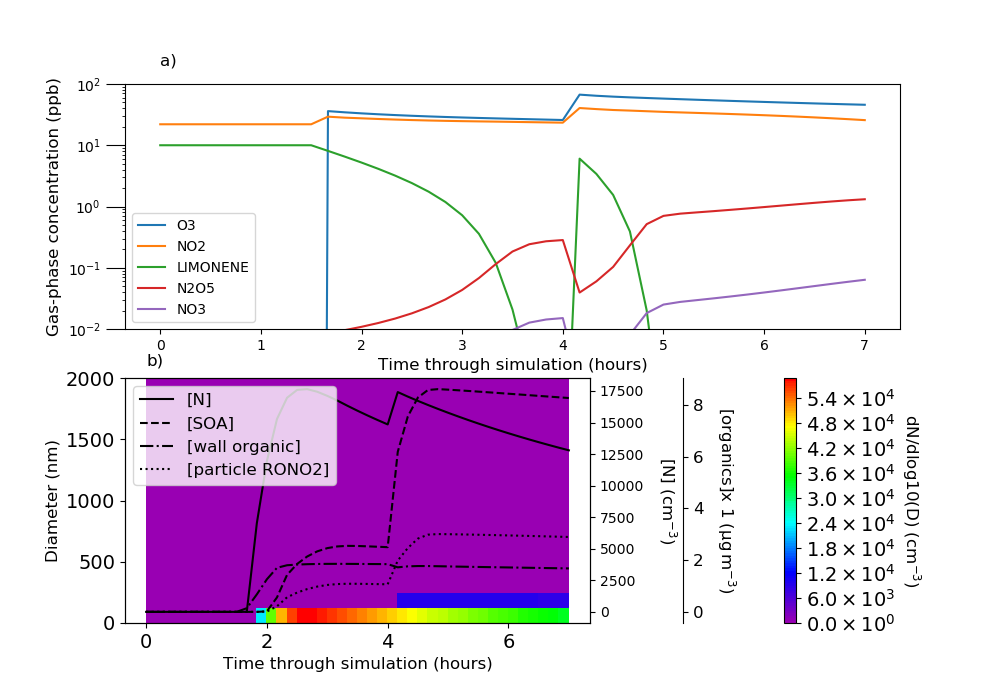
\includegraphics[width=12.0cm]{Results/limonene_res_plot.png}
\caption{Limonene oxidation in the dark with and without seed particles.  In a), the gas-phase concentrations of key components and in b), the particle properties.  At the start 10 ppb limonene, 22 ppb NO2 and 500 ppm CO are introduced.  At 1.5 hours 38 ppb O3 and 8 ppb NO2 are injected.  At 4 hours a further injection of O3 (45 ppb), limonene (10 ppb) and NO2 (19.0) is coincident with an injection of seed aerosol (10 $\mathrm{\mu g\, m^{-3}}$ with a mean radius of 0.1 $\mathrm{\mu m}$).  Particle number concentrations include seed particles, but the secondary organic aerosol mass concentration excludes the seed material.  Particle RONO2 is the sum of mass concentrations of organic components with a nitrate functional group in the particle-phase.}
\label{fig:limonene_output_plot}
\end{figure}

\section{General Structure}

For ease of navigation, PyCHAM has a modular structure with each key physicochemical process assigned to an individual module.  At the core of PyCHAM lies simultaneous numerical integration of three coupled processes: gas-phase photochemistry, vapour-particle partitioning and vapour-wall partitioning.  The ordinary differential equations (ODEs) for these processes are solved by the backward differentiation formula (which has proven reliability for these equations \citep{Jacobson2005}) from the CVODE Sundials software \citep{hindmarsh2005sundials}.  We use a python wrapper for sundials called Assimulo \citep{Andersson2015}, allowing communication between the solver and the Python code.

Coagulation, nucleation and particle loss to walls are also simulated in PyCHAM, however, because these processes are generally slower than chemical reactions and partitioning, they are operator split and solved after the integration of the ODEs mentioned above.  In the example model output of Fig.~\ref{fig:limonene_output_plot} several features of PyCHAM are demonstrated.  First, the coupling of gas-phase chemistry and resulting partitioning of vapours with sufficiently low volatility to particles and walls.  Nucleation has been simulated prior to the introduction of seed particles with approximate values given for the tuned nucleation parameters described below such that nucleation begins at the introduction of ozone, has a duration of thirty minutes and produces a peak number concentration similar to that of the seed particle.  Finally, coagulation and particle wall loss (the latter using the model of \citet{McMurry1985}), contribute to the decay in particle number concentration.

The PyCHAM software is initiated with the terminal/command window to generate a graphical user interface (GUI).  Via the GUI, users select three files  representing: i) the chemical scheme, ii) a file associating the chemical identifiers inside the chemical scheme to their Simplified Molecular Input Line Entry System (SMILE) strings \citep{Weininger1988}, and iii) a model variables file.  A fourth button on the GUI starts the simulation.

A parsing module interprets the chemical scheme and uses the chemical identifier conversion file to match component identifiers to their SMILE strings.  Additionally, modules are automatically created that will calculate time-dependent chemical reaction rates and track the rate of change of specified components.  A gas-phase initiation module sets the starting concentrations of injected components, whilst a particle-phase initiation module establishes any seed particles at experiment start.  The integration module is then called, which solves the ODEs for gas-phase photochemistry and partitioning.  Following integration, the moving-centre module is called to redistribute particles that have changed size sufficiently to cross size bin boundaries.  The coagulation and nucleation modules are the final calculations on a simulation time step before the recording time step is checked and results archived if necessary.  A saving module stores results for gas, particle and wall concentrations, corresponding time steps, particle number size distributions and constants such as component molecular weight.

The fifth and final button on the GUI will display and save graphs of the temporal profiles of number size distribution, secondary aerosol mass concentration, total particle number concentration, and the gas-phase concentrations of specified components.  If in integration mode the programme can be stopped via the terminal, or outside this mode it can be terminated by closing the GUI.

Below we describe and verify the processes described above as coded in PyCHAM.  Necessarily each process is treated in isolation, however, Fig.~\ref{fig:limonene_output_plot} and its associated text exemplify the coupling of mechanisms for a real world application.

\section{Component Properties}

The components included in the user-defined chemical scheme are automatically allocated three properties by the PyCHAM software: molecular weight, liquid density and liquid saturation vapour pressure.  Molecular weights are  estimated by passing SMILE strings to the pybel module of the Open Babel chemical toolbox \citep{OBoyle2011}.  pybel is installed as part of the PyCHAM package and generates unique chemical identifiers for each component based on their SMILE string.  For estimating component densities and liquid-phase saturation vapour pressures, the pybel chemical identifiers are passed to the UManSysProp module \citep{Topping2016} which is updated on the first run of PyCHAM and at the request of the user (via the model variables file) thereafter (requires internet connection).  By default the UMansSysProp module applies the liquid density estimation method of \citet{Girolami1994} (recommended by \citet{Barley2013}) and the liquid saturation vapour pressure estimation method of \citet{Nannoolal2008} (recommended by \citet{OMeara2014}).  Component vapour pressures have a first order effect on partitioning between phases, however estimates for certain components, particularly those with relatively low vapour pressures as these are most difficult to measure experimentally and therefore inform estimation methods,  are associated with considerable uncertainty \citep{OMeara2014}.  Consequently, users can also specify the vapour pressures of certain components.  The default particle- and wall-phase activity coefficient for all components is one, however, users may set an alternative value for specific components in the model variables folder.

\section{Gas-phase Chemistry}

For a chamber experiment including injection of reactive components, chemical reactions in the gas-phase drive the disequilibria that changes all three phases: gas, particle and wall.  As mentioned above, the Master Chemical Mechanism provides a semi-explicit model of gas-phase chemistry for several organic precursors, and developments such as PRAM express updates to our understanding.  PyCHAM is designed to accommodate such chemical schemes whilst also accepting very simplified or even empty chemical equation files.  Whilst the software manual details the requirements for input chemical schemes and chemical identifier conversion files, here we describe how PyCHAM deals with chemistry.  Equations of the general form:

\begin{equation} \label{eq:genchemreac}
s_{r_{1}}r_{1}+s_{r_{2}}r_{2} \ldots=s_{p_{1}}p_{1}+s_{p_{2}}p_{2}\ldots
\end{equation}

where $s$ represents stoichiometric number, $r$ reactants and $p$ products, are expressed as the ODEs:

\begin{align} \label{eq:genchemode}
	&\frac{d[r_{i}]}{dt} = -s_{r_{i}k_r\Pi_{j=1}^{j=n}\left([r_j]^{s_{r_{j}}}\right)}\\
	&\frac{d[p_{i}]}{dt} = s_{p_{i}k_r\Pi_{j=1}^{j=n}\left([r_j]^{s_{r_{j}}}\right)} 
\end{align}

where $n$ is the total number of reactants and $j$ is a given reactant for a given reaction.  $k_r$ is the reaction rate coefficient.

Users must therefore provide a reaction(s) of the form in Eq.~\ref{eq:genchemreac} and an associated reaction rate coefficient inside a chemical scheme file (of txt format).  Naming of chemical components inside the chemical scheme is unresticted, however, the software must be able to convert names to SMILES \citep{Weininger1988}.  Therefore, users must provide a separate file of xml format, stating a unique SMILES string for every component.  Both the chemical scheme file and the name conversion file are selected by the user via the software's GUI.

Inside the parsing module, reaction rate coefficients, reactant and product identities and their stoichiometric numbers are established from the chemical scheme file.  To separate these properties either the software's default formatting may be used, or a variant, so long as the appropriate changes are made inside the parsing module (explained in the user manual).  By default, Master Chemical Mechanism formatting is used \citep{Jenkin1997, Saunders2003}.  The Master Chemical Mechanism provides a near-explicit account of ambient atmospheric chemistry, and is presented via a user-friendly website \citep{MCM2020}.  It is recommended as a state-of-the-science resource for acquiring chemical schemes.

Reaction rate coefficients can be functions of temperature, relative humidity and concentrations of: third body, nitrogen, oxygen and peroxy radicals.  The temperature and relative humidity are input to the software by a model variables file (txt format) selected by the user via the GUI.  Third body, nitrogen and oxygen concentrations are calculated by the ideal gas law with the user-set temperature and pressure.

As in the MCM, the chemical scheme file can include generic reaction rate coefficients (those that have an identifier which is used as the reaction rate coefficient for one or more reactions).  Furthermore, the scheme can include a list of peroxy radicals, which is necessary if reaction rate coefficients are to be functions of radical concentrations.

Photochemistry is initiated through setting initial concentrations of components and stating when lights are active inside the model variables file.  The treatment of photochemistry is determined by the user and depends on the chemical scheme employed.  In the case of the Master Chemical Mechanism scheme and natural sunlight, the scattering model based on \citet{Hayman1997} and described in \citet{Saunders2003} is invoked by stating the relevant spatial and temporal coordinates in the model variables file.  For the MCM scheme and artificial lights, users must provide a file stating the wavelength-dependent actinic flux (as described in the manual).  The model then calls on the absorption cross-section and quantum yield estimates of MCM v3.3.1.  Users may provide their own absorption cross-section and quantum yield estimates



For MCM rates in natural light, users specify the: latitude, longitude, day of the year and time of day experiment commences; PyCHAM then uses the .  

For calculation of MCM photolysis rates with artificial light, a file stating actinic flux as a function of wavelength must be specified in the model variables file.  Alternatively, 

Users can also specify the components they wish to be tracked during a simulation.  PyCHAM automatically generates a module that calculates and records the rate of change of the gas-phase concentration of the given component.


\subsection{Verification}
To verify the photochemistry section of PyCHAM, gas-particle partitioning and gas-wall partitioning were turned off, leaving only gas-phase chemistry to be solved.  Here we compare against AtChem2 \citep{sommariva_acm2018} as a model benchmark.  Fig.~\ref{fig:GasChemVer1} shows the deviation with experiment time for two standard aerosol chamber characterisation experiments: alpha-pinene ozonolysis in the presence (plot a) and absence (plot b) of NOx.  To test both the dark and lit scenarios, the simulation is for an environmental chamber with an open roof, starting at midnight and finishing at midday.  Initial concentrations of $\alpha$-pinene and O$_3$ were equal at 21.1 ppb for both experiments, whilst for NOx the initial concentration was 9.8 ppb in Fig.~\ref{fig:GasChemVer1}a and 0 ppb in Fig.~\ref{fig:GasChemVer1}b.  Latitude was set to 51.51, longitude to 0.13 (London, UK) and the date was $\mathrm{1^{st}}$ July 2010.  To be comparable with AtChem2, no particle phase was present in the PyCHAM simulations and wall loss of vapours was turned off.  Deviation was calculated using:

\begin{equation} \label{eq:frac_dev}
\sigma_{i,t} = \left(\frac{s_{i,t}-b_{i,t}}{\lor(b_{i})}\right)100\mathrm{,}
\end{equation}

where $\sigma_{i,t}$ is the percentage deviation for component $i$ at time $t$, $s$ is the PyCHAM result, $b$ is the AtChem2 result and $\lor(b_{i})$ is the AtChem2 maximum for a given component during the simulation.

\begin{figure}[t]
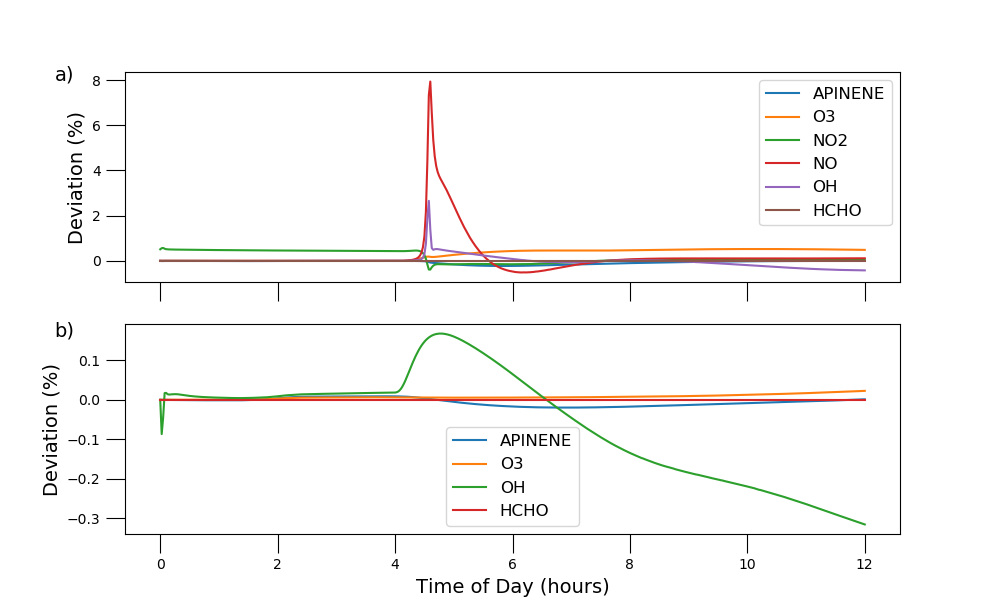
\includegraphics[width=8.3cm]{Results/photo_chem_conc_dev.png}
\caption{Gas-phase photochemistry verified; simulations of photochemistry in an aerosol chamber exposed to natural light, where deviation is defined in Eq.~\ref{eq:frac_dev}.  $\mathrm{\alpha}$-pinene ozonolysis is simulated in both plots, with $\mathrm{\alpha}$-pinene and O$_3$ given the same initial concentrations of 21.1 ppb, and initial NOx concentration in a) 9.8 ppb and in b) 0 ppb.  For both simulations, the environmental chamber is transparent and exposed to daylight without cloud interference, with dawn at approximately 4:00 hours.  The particle-phase and vapour losses to walls are turned off in PyCHAM to be consistent with the AtChem2 model.}
\label{fig:GasChemVer1}
\end{figure}

Whilst Fig.~\ref{fig:GasChemVer1} indicates that PyCHAM performs well for components with both relatively short (e.g. OH) and long (e.g. $\mathrm{\alpha}$-pinene) lifetimes, it is necessary to ascertain that agreement is gained through the correct mechanism.  Users of PyCHAM and AtChem2 can specify components that have rates of change tracked.  Such a tool is highly valuable for results analysis and trouble-shooting.  In Fig.~\ref{fig:GasChemVer2} we use it to compare the reaction rates for formaldehyde for the same $\mathrm{\alpha}$-pinene ozonolysis simulations used for Fig.~\ref{fig:GasChemVer1}.  The deviations were again calculated using Eq.~\ref{eq:frac_dev}, but with concentrations replaced by gas-phase concentration rate of change.  Of the loss and production reactions for formaldehyde the two of each with greatest deviation are shown in Fig.~\ref{fig:GasChemVer2}.  The close agreement with AtChem2 results in Fig.~\ref{fig:GasChemVer1} demonstrates that PyCHAM indeed integrates gas-phase photochemistry correctly.

\begin{figure}[t]
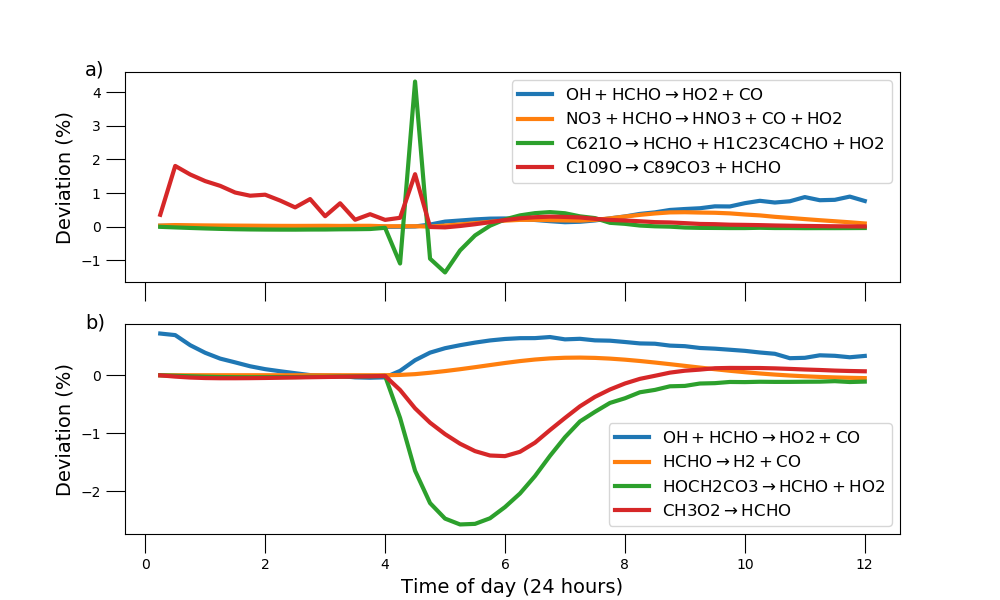
\includegraphics[width=8.3cm]{Results/photo_chem_grad_dev.png}
\caption{Deviation of PyCHAM simulated rate of change of formaldehyde (HCHO) due to the MCM reactions given in the legends versus AtChem2 simulations.  Where the definition for deviation is given in Eq.~\ref{eq:frac_dev}.  Both plots are results for the $\alpha$-pinene ozonolysis reaction described in the main text for Fig.~\ref{fig:GasChemVer1}, with a) is in the presence of NOx and b) is in the absence of NOx.}
\label{fig:GasChemVer2}
\end{figure}


\subsection{Sensitivity to temporal resolution}

For minimising wall-clock time, users can increase the maximum time step for integration of the photochemical problem in Eq.~\ref{eq:genchemode}.  Clearly, increases in time step lead to loss of temporal detail, therefore the user must balance the need for reduced wall-clock time against loss of accuracy in simulated gas-phase concentrations.  In Fig.~\ref{fig:GasChemTimeRes} the effect of increasing integration time step by an order of magnitude from $\mathrm{6x10^2}$ s to $\mathrm{6x10^3}$ s on gas-phase concentration changes is shown and demonstrates loss of accuracy.  Deviation was calculated by replacing AtChem2 inputs to Eq.~\ref{eq:frac_dev} with simulated results from PyCHAM at a 60 s resolution.  Users are advised to conduct a similar test if their chemical scheme or environmental conditions vary significantly from those here.

\begin{figure}[t]
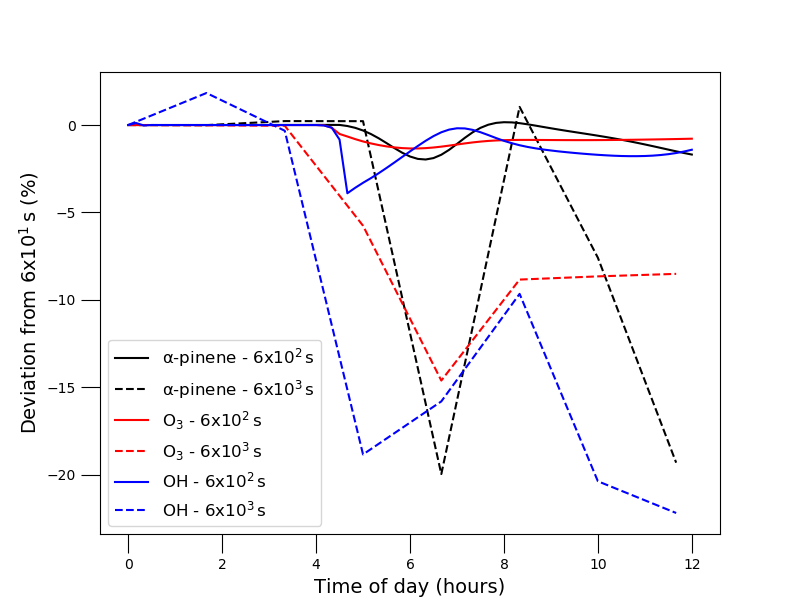
\includegraphics[width=8.3cm]{Results/photo_chem_time_res.png}
\caption{Illustrating the effect of model time resolution in PyCHAM on gas-phase concentrations of $\alpha$-pinene, $\mathrm{O_3}$ and OH for the $\mathrm{\alpha}$-pinene ozonolysis in presence of NOx experiment described above for Fig.~\ref{fig:GasChemVer1}.  The integration time steps were set to $\mathrm{6x10^2}$ and $\mathrm{6x10^3}$ s as shown in the legend, and the deviation is that from results for an integration step of $\mathrm{6x10^1}$ s.}
\label{fig:GasChemTimeRes}
\end{figure}

\section{Gas-wall partitioning}

The partitioning of gases to the chamber wall is often termed wall loss as the net movement is from the gas phase to the wall (for an initially clean chamber wall).  Traditionally this process has been viewed as an inconvenience since chamber results often depend on the concentration of gas- and particle-phases of certain components, whilst the fraction of these components lost to walls is poorly constrained.  Several studies have focussed on partitioning to Teflon walls, which are frequently employed \citep{Matsunaga2010, Zhang2015b, Zhao2018}, however, the process remains poorly modelled across the wide range of chamber materials, relative humidities, gas-phase loading, component volatilities and activity coefficients present in chamber experiments \citep[e.g.][]{Day2017, Stefenelli2018}.  It is therefore preferable to allow the user to fit vapour losses to walls through the tuning of two wall loss parameters, one primarily determining equilibrium, called the effective wall mass concentration ($C_w$), and one determining rate of partitioning, the mass transfer coefficient ($k_w$).  These influence gas-wall partitioning through an equation of the same framework as gas-particle partitioning \citep{Zaveri2008}:

\begin{align} \label{eq:gas_wall_partit}
	&\frac{dC_{i,g}}{dt} = -k_{w}(C_{i,g}-\frac{C_{i,w}}{C_{w}}p^{0}_{i}\gamma_{i})\rm{,}\\
	&\frac{dC_{i,w}}{dt} = k_{w}(C_{i,g}-\frac{C_{i,w}}{C_{w}}p^{0}_{i}\gamma_{i})\rm{,}
\end{align}

where $p^{0}_{i}$ is the liquid-phase saturation vapour pressure of component $i$ and $\gamma_{i}$ is its activity coefficient on the wall.  Following the conclusions of \citet{Matsunaga2010} and \citet{Zhang2015b}, $k_{w}$ represents factors such as gas- and wall-phase diffusion, turbulence, accommodation coefficient and the chamber surface area to volume ratio, whilst $C_{w}$ reflects the absorbing and adsorbing properties of the wall, including relative humidity, surface area, diffusivity and porosity.  For chambers and systems where these factors have not been probed, we recommend the iterative fitting of $k_{w}$ and $C_{w}$ to observations through minimising observation-model residuals.

A major distinction between the gas partitioning to particles and walls is the much greater size of the wall, where size is represented by surface area or volume depending on whether adsorption or absorption is the main partitioning mechanism, respectively.  It could be argued that the effective wall mass concentration is massive compared to the concentration of wall-phase components, making the Raoult (mole fraction ($\frac{C_{i,w}}{C_{w}}$)) term in Eq.~\ref{eq:gas_wall_partit} redundant.  Following this argument, the gas-wall partitioning equation becomes:

\begin{equation} \label{eq:gas_wall_partit2}
\frac{dC_{i,g}}{dt} = -k_{w}(C_{i,g}-\frac{p^{0}_{i}\gamma_{i}}{C_{w}})\rm{.}
\end{equation}

However, this approach is unphysical as it removes the dynamic property of partitioning, instead, the $\frac{p^{0}_{i}\gamma_{i}}{C_{w}}$ term implies a fixed concentration of wall-phase component in the gas-phase just above the wall and introduces several issues.  First, it suggests that components with higher volatility and lower activity coefficient have a greater concentration on the wall which is unrealistic.  Second, the fixed wall concentration allows for loss of mass conservation for components with $C_{i,g}<\frac{p^{0}_{i}\gamma_{i}}{C_{w}}$ since components may evaporate from the wall despite having no presence there.  Conversely, components with  $C_{i,g}>\frac{p^{0}_{i}\gamma_{i}}{C_{w}}$ may undergo an unrealistic degree of condensation to the wall because the evaporation of their wall-phase is unaccounted for.

Next we illustrate the sensitivity to and $k_{w}$ and $C_{w}$ in Eq.~\ref{eq:gas_wall_partit}.  The same simulation setup described above for Fig.~\ref{fig:GasChemVer1} was used though with $\mathrm{\alpha}$-pinene replaced by isoprene with a concentration at experiment start of 63.4 ppb and including seed particle comprised of a non-volatile component (ammonium sulphate) with mean diameter 0.5 $\mathrm{\mu m}$ and number concentration $\mathrm{6x10^{2}\; cm^{-3}}$.  Pure component liquid saturation vapour pressures were estimated by the \citet{Nannoolal2008} method and activity coefficients for all components were assumed one.  To begin, both $k_{w}$ and $C_{w}$ were set sufficiently low to effectively turn off gas-wall partitioning.  Second, $C_{w}$ was set equal to the mass concentration of seed particle (70 $\mathrm{\mu g\,m^{-3}}$) and $k_{w}$ raised to $\mathrm{1x10^{-1}\, s^{-1}}$ at which a notable decrease in [SOA] was observed.  Third, $k_{w}$ was held whilst $C_{w}$ was raised three orders of magnitude greater than the seed mass concentration.  Fourth, $C_{w}$ was held at 70 $\mathrm{\mu g\,m^{-3}}$ and $k_{w}$ was raised by three orders of magnitude.  The effect on produced secondary organic aerosol mass concentration is given in Fig.~\ref{fig:Gaswall_sens_fig} and demonstrates that at sufficiently large values of $C_{w}$, SOA production can be effectively suppressed through competitive uptake of vapours to chamber walls.  However, for a given $C_{w}$, there is a limit on suppression of SOA formation due to $k_{w}$ increase as it affects only the rate of partitioning with walls rather than the degree of partitioning.

To guide constraint for wall loss parameters, we follow the example of \citet{Matsunaga2010} with a control experiment comprising a single semi-volatile component introduced to the chamber at the start of the simulation at 50 ppb.  We chose 2-methylglyceric acid which has an estimated particle mass concentration saturation vapour pressure ($C*$) of 115 $\mathrm{\mu g\,m^{-3}}$ at 298.15 K (the temperature in the simulation) and is an observed oxidation product of isoprene \citep{Surratt2006}.  No other components or particles are introduced.  With regards to designing a control experiment for tuning $C_{w}$ and $k_{w}$, the results shown in Fig.~\ref{fig:Gaswall_sens_fig}b demonstrate that a component with a $C*$ close to the $C_{w}$ has large sensitivity to the $C_{w}$ value, thereby allowing greatest ease of tuning.  Note, that this sensitivity can be altered through varying chamber temperature (and therefore the $C*$ of a component), or through varying component.  Furthermore, to discern the effect of $k_{w}$ a component with substantial partitioning to walls is required.  When quantifying $k_{w}$ it is worthwhile considering the required precision, because as Fig.~\ref{fig:Gaswall_sens_fig}a demonstrates, above a certain value, no further effect on SOA concentration results.

\begin{figure}[t]
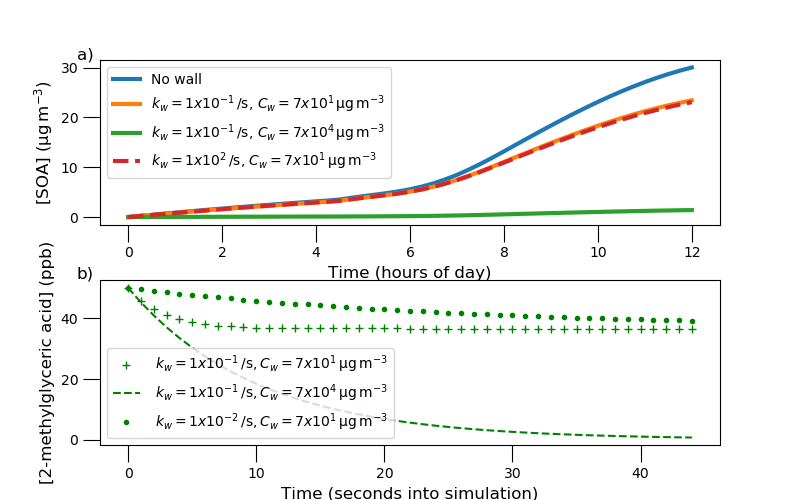
\includegraphics[width=8.3cm]{Results/Gaswall_sens_fig.png}
\caption{In a) sensitivity of secondary organic aerosol mass concentration on the gas-wall partitioning parameters $k_{w}$ and $C_{w}$ from Eq.~\ref{eq:gas_wall_partit}.  Seed particles with a concentration of approximately 70 $\mathrm{\mu g\, m^{-3}}$ were present at the start of the experiment.  Initial concentrations of ozone, isoprene and $\mathrm{NO_{2}}$ were set to 21.1, 63.4 and 9.8 ppb, respectively.  With regards to photolysis rates, the simulation made the same considerations as in Fig.~\ref{fig:GasChemVer1}, where natural sunlight drove reactions after dawn at approximately 4:00 am.  In b), the same sensitivity is assessed, but for a control experiment where only a single organic component is present in the gas phase.}
\label{fig:Gaswall_sens_fig}
\end{figure}

\section{Evolution of particle size distribution}

Simulations, like chamber experiments, are possible with and without seed particles.  For seed particle experiments, the user defines their number size distribution and composition inside the model variables input file.  Furthermore, because PyCHAM uses size bins to discretise particles, users can state the number of size bins, lower and upper bin bounds and whether they would like the bins to be spread linearly or logarithmically in radius space.  

Once the number-size distributions are initiated, three processes modelled by PyCHAM can directly cause particles to shrink or grow: gas-particle partitioning, coagulation and nucleation.  The former two use established equations and therefore are not repeated here.  Whilst coagulation and nucleation are discussed below, readers are referred to \citet{Zaveri2008} for a thorough explanation of gas-particle partitioning.  The transition regime correction factor required for the partitioning estimation in PyCHAM is from \citet{Fuchs1971}.  Furthermore, users can use the module $\rm{test\_kimt\_calc}$ to check that the Kelvin and Raoult effects of the PyCHAM partitioning equation are accurate (e.g. through comparison with Fig. 16.1 of \citet{Jacobson2005}).

In this section we focus on redistribution of particles between size bins following a change in size.  PyCHAM does this using the moving-centre structure \citep{Jacobson2005}.  The moving-centre approach has the advantage of minimal numerical diffusion, however, it suffers from loss of particle history due to its combining of mass of particles originally from varying size bins \citep{Zhang1999}.  The user must consider this weakness when determining whether the model is suitable for their purpose.  To maintain stability in numerical solutions and improve model accuracy, a condition inside the moving centre module of PyCHAM iteratively reduces the integration time step if particles in a size bin change volume sufficiently to be allocated to a size bin beyond the adjacent one.  If this condition is not met again, the integration step will be doubled every ten steps until it returns to the maximum set by the user.

Here we assess the moving-centre method through analysis of output during two relatively intense (and therefore testing) periods of vapour-particle partitioning and compare to benchmark simulations.  The simulations also illustrate two further means of component influx to chambers using PyCHAM in addition to the simulations above where components were introduced with an initial pulse.  In the first case a constant flux of sulphuric acid is added to a chamber with seed aerosol typical of hazy conditions following the benchmark simulation of \citet{Zhang1999}.  For consistency with the benchmark, vapour and particle partitioning to walls was turned off and sulphuric acid was assumed to be non-volatile.  In their analysis \citet{Zhang1999} remark that to resolve the growth of smallest particles in this scenario spatial resolution must be at least 100 size bins, therefore we chose this value and set the solution time interval to 90 s for a total 12 hour simulation.  The exact solution to this condensational growth problem is given in Fig.~\ref{fig:mov_cen_test}a) (taken from Fig. 3 of \citet{Zhang1999}) and is provided by the full-moving structure.  When PyCHAM is compared against the exact solution, the tri-modal distribution is present with mean values at the correct particle size though with some disagreement in the peak height and spread.  The degree of agreement is significantly better than for the 13 size bin moving-centre simulation presented in \citet{Zhang1999} and indicates that PyCHAM is operating as intended.  Our results in Fig.~\ref{fig:mov_cen_test}a) are a two-point moving average which is often necessary for the moving-centre structure because its requirement that all particles in a size bin be transferred to the adjacent bin means that some bins will intermittently have zero particles.

Another case of relatively intense vapour-particle partitioning is provided by the example of cloud condensation nuclei experiencing varying degrees of water vapour supersaturation.  Chamber experiments may involve injections of a component at specific times and the model variables input file is able to carry this information to PyCHAM.  Making use of this function we reproduce the benchmark simulation of \citet{Jacobson2005} (Fig. 13.8) where relative humidity is increased to 100.002 \% every minute (including at simulation start) for nine minutes, with results analysed after ten minutes.  Seed particles are assumed non-volatile and wall interactions are turned off.  Parameters such as temperature and the degree of dissociation, molecular weight and density of the seed particle are not disclosed by the reference simulation, therefore we set these as: 318.15 K, 1.0, 200 $\mathrm{g\,mol^{-1}}$ and 1 $\mathrm{g\,cm^{-3}}$, respectively.  The comparison between the \citet{Jacobson2005} result in Fig.~\ref{fig:mov_cen_test}b) and PyCHAM certainly shows agreement in the main feature of this simulation, which is the initially larger particles out competing smaller particles for water condensation to grow to water droplet size ($D_{p}>10\, \mathrm{\mu m}$).  The PyCHAM result gives reasonable agreement considering that key parameters (such as seed component dissociation) may vary between simulations.

\begin{figure}[t]
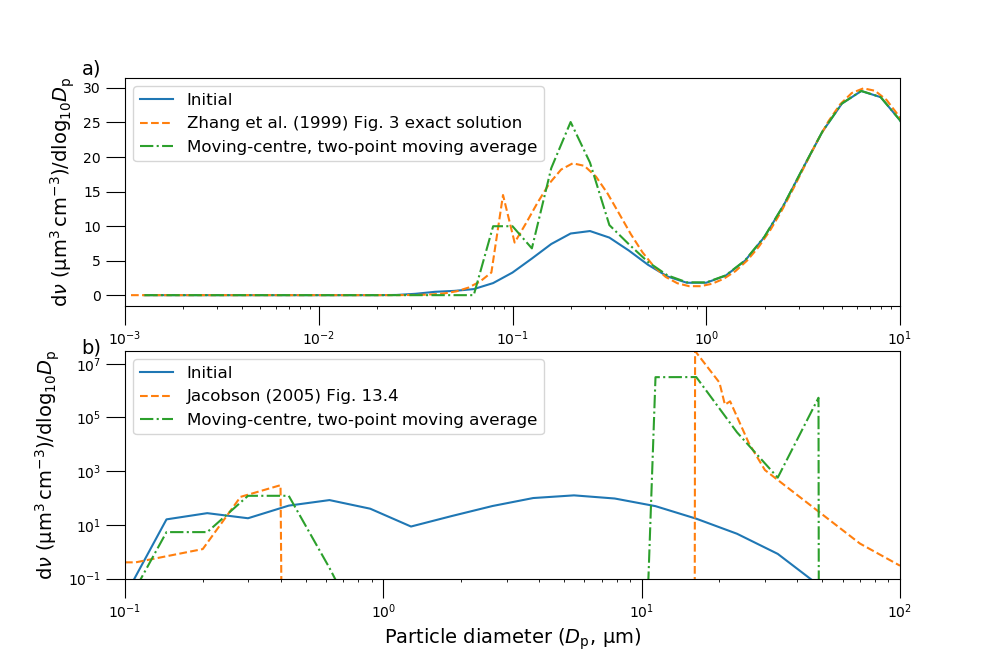
\includegraphics[width=10.0cm]{Results/mov_cen_test.png}
\caption{In a), replication of Fig.3 of \citet{Zhang1999} where a constant influx of sulphuric acid condenses to seed particles with the shown initial volume-size distribution, with final results shown after 12 hours.  In b), replication of Fig. 13.8 of \citet{Jacobson2005}, where an initial distribution of particles are subject to a relative humidity of 100.002 \% at minute intervals for 9 minutes, with results shown after 10 minutes.}
\label{fig:mov_cen_test}
\end{figure}

\section{Coagulation}

Equations of coagulation kernels for Brownian diffusion, convective Brownian diffusion enhancement, gravitational collection, turbulent inertial motion, turbulent shear and Van der Waals collision were taken from \citet{Jacobson2005}.  The module $\rm{test\_coag}$ produces a plot of coagulation kernels that can be compared to Fig. 15.7 of \citet{Jacobson2005} to verify its accuracy.  Once the cumulative coagulation kernel for each pair of particle size bins ($\beta$) has been found, the combinations of size bins (denoted $j$ and $z$) whose coagulation produces a particle of size bin $k$ are identified:

 \begin{equation} \label{eq:coag2}
Vb_{l,k} \leq (V_{j,t-h}+V_{z,t-h}) < Vb_{u,k},
\end{equation}

where $V$ is particle volume, $Vb_{l,k}$ and $Vb_{u,k}$ are the lower and upper volume bounds of the size bin and $h$ is the time step for coagulation to occur over.  The semiimplicit coagulation equation from \citet{Jacobson2005} is then used to estimate the new number concentration per size bin ($N$ $(\#\, \mathrm{cm^{-3}})$):

\begin{equation} \label{eq:coag1}
N_{k,t} = \frac{N_{k,t-h}+\frac{1}{2}h\sum_{j=1}^{j_{max}}\beta_{z,j}N_{z,t}N_{j,t-h}}{1+h\sum_{j=1}^{\infty}\beta_{k,j}N_{j,t-h}},
\end{equation}

where $j_{max}$ is the largest size bin that can undergo coagulation to produce a particle in size bin $k$.  This equation is not mass-conserving, however, the mass transfer between size bins is estimated using the number fraction of particles coagulating.  For example, for a size bin $k$, the gain in molecular concentration of component $i$ due to coagulation between size bins $j$ and $z$ (according to Eq.~\ref{eq:coag2} and Eq.~\ref{eq:coag1}):

\begin{equation} \label{eq:coag3}
\Delta C_{i,k} = \frac{h(\frac{1}{2}\beta_{z,j}N_{z,t}N_{j,t-h}+\frac{1}{2}\beta_{j,z}N_{j,t}N_{z,t-h})}{N_{j,t-h}}C_{i,j,t-h},
\end{equation}

and the loss of molecular concentration from size bin $k$ due to coagulation is:

\begin{equation} \label{eq:coag4}
\Delta C_{i,k} = -\left(1-\frac{1}{1+h\sum_{j=1}^{\infty}\beta_{k,j}N_{j,t-h}}\right)C_{i,k,t-h},
\end{equation}

Eqs.~\ref{eq:coag1}-~\ref{eq:coag4} show that coagulation directly influences the particle number and mass size distributions.  Here, we asses the sensitivity of the number size distribution and mass conservation to temporal and spatial resolution.  A relatively complex initial distribution with four number modes is taken from ambient observations at Claremont, California on August 27, 1987 \citep{Jacobson2005} and assumed to comprise non-volatile material.  Results are presented for a six hour simulation in Fig.~\ref{fig:coag_resol_test_plot} where particle wall loss was turned off to allow clearer assessment of the coagulation sensitivity.  In the top row of Fig.~\ref{fig:coag_resol_test_plot} no gas-phase chemistry was allowed, whilst in the bottom row, a single chemical reaction with reaction rate $\mathrm{5.6x10^{-17}\, molec^{-1}s^{-1}}$  between $\mathrm{\alpha-}$pinene and ozone (both with initial concentrations 100 ppb) was modelled to produce a single low volatility product with saturation vapour pressure of $\mathrm{1x10^{-10}}$ Pa, whilst gas-wall partitioning was turned off.  For the chemistry case, approximately 500 $\mathrm{\mu g\, m^{-3}}$ of secondary material was formed, compared to  90 $\mathrm{\mu g\,m^{-3}}$ of seed material.  Columns in Fig.~\ref{fig:coag_resol_test_plot} are distinguished by the size bin resolution as presented in the column titles, and in each plot temporal resolutions are varied.

The inset text of Fig.~\ref{fig:coag_resol_test_plot} ($\Delta nv$) gives the fractional change in non-volatile material from the start to end (six hours) of the simulation for the three temporal resolutions.  It is clear that the coagulation equations given introduce a negligible error in mass conservation.  Two features are present in the top row (no chemistry) of Fig.~\ref{fig:coag_resol_test_plot}: first, that coagulation overwhelmingly affects the number concentration of smaller particles - note that such particles are sufficiently small in volume that they may coagulate with a larger particle without causing it to grow a size bin; second, that only for the smallest particles (below a diameter of $\mathrm{3x10^{-2}\; \mu m}$ in this case) is a sensitivity to temporal resolution clear across all size bin resolutions.  Regarding spatial resolution for the no chemistry case, an increase allows greater precision of the effect on smaller particles, which also results in a greater loss of accuracy when using lower temporal resolution.  However, all the resolution considerations above become redundant when we consider the case with gas-particle partitioning of secondary species (bottom row of Fig.~\ref{fig:coag_resol_test_plot}).  In this instance, the effect of partitioning dominates the change in number-size distribution and no sensitivity of coagulation to spatial or temporal resolution is discernible.  We recommend users consider these examples in addition to the nature of their simulation and objective when deciding whether temporal or spatial resolution will significantly impact results.

\begin{figure}[t]
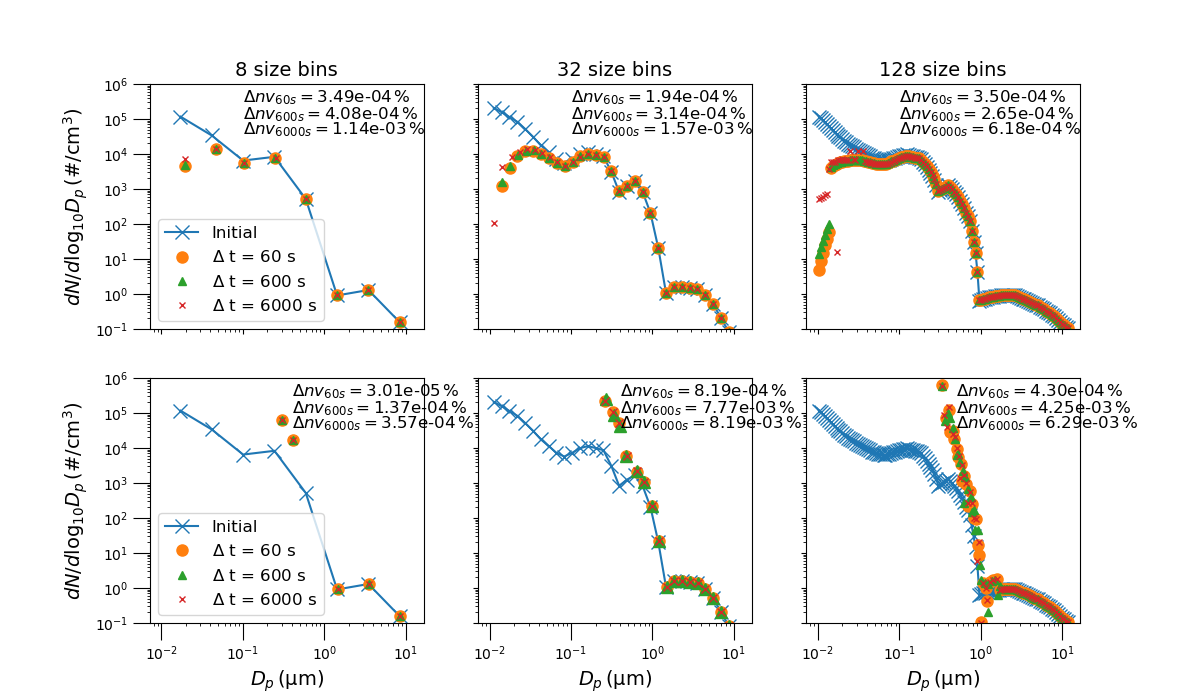
\includegraphics[width=12.0cm]{Results/coag_resol_test_plot.png}
\caption{Sensitivity of the coagulation process to changes in temporal resolution (given in the legend) and spatial resolution (given in column titles).  In the top row no chemistry occurred whilst in the bottom row a semi-volatile species was produced, as detailed in the main text.  Results are for the end of a simulated six hour experiment.  The $\Delta nv_{\mathrm{temporal\; resolution}}$ value given in the inset text is the percentage change in total non-volatile particle-phase material from the start to finish of the experiment, demonstrating mass conservation in the model.}
\label{fig:coag_resol_test_plot}
\end{figure}

\section{Particle deposition to walls}

As with gas-wall partitioning, the loss of particles to chamber walls can significantly invalidate chamber results if unaccounted for and has been detailed in previous publications \citep{McMurry1985, Nah2017, Wang2018}.  During control experiments the deposition rate of particles to walls can be inferred through observations of the rate of decay of particles of varying size (with coagulation accounted for) \citep{Charan2019}.  Several studies have published results from such experiments \citep{McMurry1985, Wang2018}, including a relatively large dataset from the EUROCHAMP2020 project \citep{EUROCHAMP2020}.  Comparison of inferred wall loss rates indicate that relatively small and larger particles have higher loss rates due diffusion and settling, respectively, however the absolute values and size-dependent gradient of the loss rates vary significantly between control experiments.  Even for a given chamber significant variations appear with changes to relative humidity, disturbance to walls due to air conditioning, and, for teflon chambers, with time since the chamber walls experienced frictional force to create electrostatic charge.  Currently no method is available to measure the required inputs that a particle deposition model would need to satisfactorily reproduce observations, therefore in PyCHAM users have three options to estimate particle wall deposition.  Here we describe the options and provide examples of their use.

Users select wall loss treatment with the McMurry\_flag option in the model variables input file.  The default (if left empty) is no loss of particles to wall.  If set to 1, the model of \citet{McMurry1985} is used, which is based on the particle deposition model of \citet{Crump1981} but with electrostatic effects.  Studies have found the \citet{Crump1981} and \citet{McMurry1985} approach to reproduce measured particle wall losses well \citep{Chen1992, Kim2001}.  Selecting \citet{McMurry1985} requires the user to also input the chamber surface area, the average charge per particle and the average electric field inside the chamber, where the latter two may be set to zero for nullifying electrostatic effects.  With the $\rm{test\_wallloss}$ module users can confirm that PyCHAM accurately reproduces Fig. 2 of \citet{McMurry1985}, as shown here in Fig.~\ref{fig:part_wall_depo_plot}, which demonstrates the effect of changing the charge number per particle.

If user sets the McMurry\_flag option to 0 then a customised particle deposition rate dependence on particle size is available.  This option allows users to transfer measured deposition rates to the model, as recommended by \citet{Wang2018}.  Four further inputs are required for this option: the particle diameter at which the inflection in deposition rates occurs ($D_{p,flec}$), where the inflection point marks a change in dependance of deposition rate with particle size, the rate of particle deposition to wall at the inflection point ($\beta_{flec}$), and the gradients of the deposition rate with respect to particle diameter before ($\nabla_{pre}$) and after the inflection ($\nabla_{pro}$), where a linear dependence in log-log space is assumed, consistent with observations \citep{Charan2019}.  The employed equations for deposition rate in this instance are given in Eq.~\ref{eq:man_part_wl}, and example dependencies of rate with particle size provided by Fig.~\ref{fig:part_wall_depo_plot}.

\begin{align} \label{eq:man_part_wl}
D_{p}<D_{p,flec} \nonumber \\
&\rm{log_{10}}(\mit{\beta(D_{p}})) = \rm{log_{10}}(\mit{D_{p,flec}})-\rm{log_{10}}\mit{(D_{p})}\nabla_{pre}+\beta_{flec} \nonumber \\
D_{p}\geq D_{p,flec} \nonumber \\
&\rm{log_{10}}(\mit{\beta(D_{p}})) = \rm{log_{10}}(\mit{D_{p}})-\rm{log_{10}}\mit{(D_{p,flec})}\nabla_{pro}+\beta_{flec}
\end{align}

\begin{figure}[t]
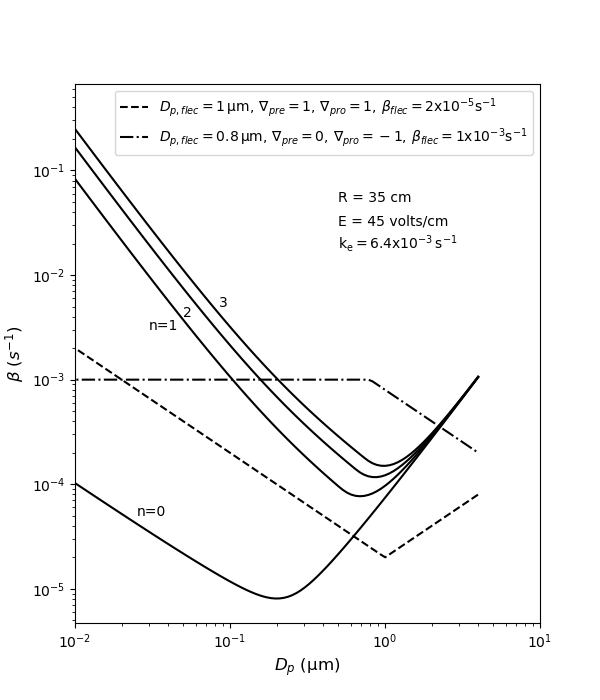
\includegraphics[width=8.3cm]{Results/part_wall_depo_plot.png}
\caption{Example dependencies of the particle deposition to wall rate using the model of \citet{McMurry1985} in the solid lines, where the charge per particle is given by n and other inputs given by inset text (R is spherical-equivalent chamber radius, E is the average electric field in the chamber) and $\mathrm{k_e}$ is the coefficient of eddy diffusion.  The dashed lines demonstrate the the observation-based deposition rate utility of PyCHAM given in Eq.~\ref{eq:man_part_wl}, with inputs at the top of the plot.}
\label{fig:part_wall_depo_plot}
\end{figure}

\section{Nucleation}

The simulation of nucleation to produce newly-formed suspended particles is an area of ongoing research \citep[e.g.][]{Kurten2018, Semeniuk2018, Li2020}.  To date, there is not a generally acceptable model.  Consequently, for PyCHAM simulations involving nucleation, users are able to provide parameters to a Gompertz function, allowing them to fit to observed number size distributions:

\begin{equation} \label{eq:Gompertz}
P_{1}(t) = \rm{nuc_{v1}}\left(\exp \left(\rm{nuc_{v2}}\left(\exp \left(\mit{-t}/\rm{nuc_{v3}} \right) \right) \right) \right)
\end{equation}

where $P_{1}$ is the number concentration of new particles after time $t$ that enter the smallest size bin, and $\rm{nuc_{vn}}$ are the user-defined parameters.  The resulting function forms a sigmoidal curve with time, whilst the parameters allow the amplitude ($\rm{nuc_{v1}}$), onset ($\rm{nuc_{v2}}$), and duration ($\rm{nuc_{v3}}$) of the curve to be adjusted, as shown in Fig. ~\ref{fig:nuc_sens}

\begin{figure}[t]
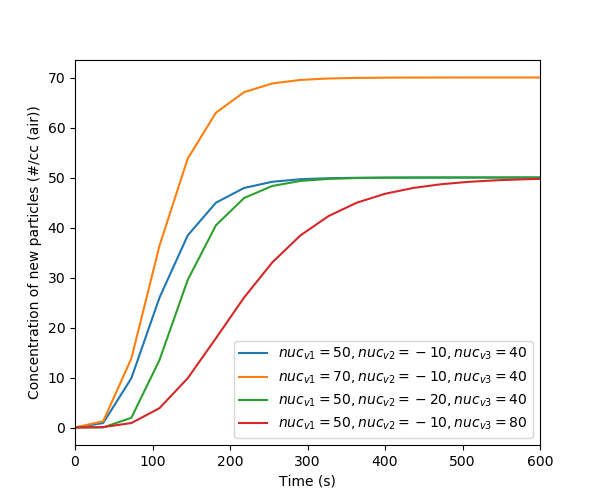
\includegraphics[width=8.3cm]{Results/nuc_sens.png}
\caption{Effect of varying the nucleation parameters.}
\label{fig:nuc_sens}
\end{figure}

To obtain the nucleation parameters that most accurately fit measurements, number size distribution measurements provide a relatively detailed indicator of fit, whilst total particle number concentration is less informative and therefore less able to provide constraint.

Although it is accepted that clusters of molecules are responsible for forming the nucleus of a particle \citep{Seinfeld2006}, the shape and spherical-equivalent radius of these is unknown.  Inside PyCHAM, newly nucleated particles are assigned a radius provided by the user in the model inputs file.  Using the volume equation for the cluster's assumed spherical shape and the molar volume of the component assumed responsible for nucleation (also prescribed by the user), the molar concentration of nucleating component required is calculated and added to the smallest size bin of the particle phase whilst subtracted from the vapour phase.  The average radius of the particles in this size bin is then calculated by dividing the total volume of molecules by the number of particles.


\conclusions  %% \conclusions[modified heading if necessary]
The PyCHAM (CHemistry with Aerosol Microphysics in Python) model for aerosol chambers has been described.  It is novel in its ease of accessibility and use.  Key features including gas-phase photochemistry, gas-particle partitioning, gas-wall partitioning, redistribution of particles between size bins, coagulation, wall loss of particles and nucleation have been demonstrated, and where relevant, verified against benchmark simulations.  Whilst aerosol chambers may be used in a variety of manners, the model variables input file allows these to be described in one place with a versatility that has been illustrated in the examples given.  Finally the effect of decreasing temporal and spatial resolution on relevant processes has been demonstrated.L

%% The following commands are for the statements about the availability of data sets and/or software code corresponding to the manuscript.
%% It is strongly recommended to make use of these sections in case data sets and/or software code have been part of your research the article is based on.

\codeavailability{TEXT} %% use this section when having only software code available
Code available here: https://github.com/simonom/PyCHAM - and DOI will be allocated once the JOSS paper is published.


\dataavailability{TEXT} %% use this section when having only data sets available


\codedataavailability{TEXT} %% use this section when having data sets and software code available


\sampleavailability{TEXT} %% use this section when having geoscientific samples available


\videosupplement{TEXT} %% use this section when having video supplements available


\appendix
\section{}    %% Appendix A

\subsection{}     %% Appendix A1, A2, etc.


\noappendix       %% use this to mark the end of the appendix section

%% Regarding figures and tables in appendices, the following two options are possible depending on your general handling of figures and tables in the manuscript environment:

%% Option 1: If you sorted all figures and tables into the sections of the text, please also sort the appendix figures and appendix tables into the respective appendix sections.
%% They will be correctly named automatically.

%% Option 2: If you put all figures after the reference list, please insert appendix tables and figures after the normal tables and figures.
%% To rename them correctly to A1, A2, etc., please add the following commands in front of them:

\appendixfigures  %% needs to be added in front of appendix figures

\appendixtables   %% needs to be added in front of appendix tables

%% Please add \clearpage between each table and/or figure. Further guidelines on figures and tables can be found below.



\authorcontribution{TEXT} %% this section is mandatory

\competinginterests{TEXT} %% this section is mandatory even if you declare that no competing interests are present

\disclaimer{TEXT} %% optional section

\begin{acknowledgements}

This project has received funding from the European Union's Horizon 2020 research and innovation programme under grant agreement No 730997.

\end{acknowledgements}




%% REFERENCES

%% The reference list is compiled as follows:
\bibliographystyle{copernicus}
\bibliography{Bibtex_refs}
\begin{thebibliography}{}




\end{thebibliography}

%% Since the Copernicus LaTeX package includes the BibTeX style file copernicus.bst,
%% authors experienced with BibTeX only have to include the following two lines:
%%
%% \bibliographystyle{copernicus}
%% \bibliography{example.bib}
%%
%% URLs and DOIs can be entered in your BibTeX file as:
%%
%% URL = {http://www.xyz.org/~jones/idx_g.htm}
%% DOI = {10.5194/xyz}
%%\bibitem[AUTHOR(YEAR)]{LABEL1}
%%REFERENCE 1
%%
%%\bibitem[AUTHOR(YEAR)]{LABEL2}
%%REFERENCE 2

%% LITERATURE CITATIONS
%%
%% command                        & example result
%% \citet{jones90}|               & Jones et al. (1990)
%% \citep{jones90}|               & (Jones et al., 1990)
%% \citep{jones90,jones93}|       & (Jones et al., 1990, 1993)
%% \citep[p.~32]{jones90}|        & (Jones et al., 1990, p.~32)
%% \citep[e.g.,][]{jones90}|      & (e.g., Jones et al., 1990)
%% \citep[e.g.,][p.~32]{jones90}| & (e.g., Jones et al., 1990, p.~32)
%% \citeauthor{jones90}|          & Jones et al.
%% \citeyear{jones90}|            & 1990



%% FIGURES

%% When figures and tables are placed at the end of the MS (article in one-column style), please add \clearpage
%% between bibliography and first table and/or figure as well as between each table and/or figure.


%% ONE-COLUMN FIGURES

%%f
%\begin{figure}[t]
%\includegraphics[width=8.3cm]{FILE NAME}
%\caption{TEXT}
%\end{figure}
%
%%% TWO-COLUMN FIGURES
%
%%f
%\begin{figure*}[t]
%\includegraphics[width=12cm]{FILE NAME}
%\caption{TEXT}
%\end{figure*}
%
%
%%% TABLES
%%%
%%% The different columns must be seperated with a & command and should
%%% end with \\ to identify the column brake.
%
%%% ONE-COLUMN TABLE
%
%%t
%\begin{table}[t]
%\caption{TEXT}
%\begin{tabular}{column = lcr}
%\tophline
%
%\middlehline
%
%\bottomhline
%\end{tabular}
%\belowtable{} % Table Footnotes
%\end{table}
%
%%% TWO-COLUMN TABLE
%
%%t
%\begin{table*}[t]
%\caption{TEXT}
%\begin{tabular}{column = lcr}
%\tophline
%
%\middlehline
%
%\bottomhline
%\end{tabular}
%\belowtable{} % Table Footnotes
%\end{table*}
%
%%% LANDSCAPE TABLE
%
%%t
%\begin{sidewaystable*}[t]
%\caption{TEXT}
%\begin{tabular}{column = lcr}
%\tophline
%
%\middlehline
%
%\bottomhline
%\end{tabular}
%\belowtable{} % Table Footnotes
%\end{sidewaystable*}
%
%
%%% MATHEMATICAL EXPRESSIONS
%
%%% All papers typeset by Copernicus Publications follow the math typesetting regulations
%%% given by the IUPAC Green Book (IUPAC: Quantities, Units and Symbols in Physical Chemistry,
%%% 2nd Edn., Blackwell Science, available at: http://old.iupac.org/publications/books/gbook/green_book_2ed.pdf, 1993).
%%%
%%% Physical quantities/variables are typeset in italic font (t for time, T for Temperature)
%%% Indices which are not defined are typeset in italic font (x, y, z, a, b, c)
%%% Items/objects which are defined are typeset in roman font (Car A, Car B)
%%% Descriptions/specifications which are defined by itself are typeset in roman font (abs, rel, ref, tot, net, ice)
%%% Abbreviations from 2 letters are typeset in roman font (RH, LAI)
%%% Vectors are identified in bold italic font using \vec{x}
%%% Matrices are identified in bold roman font
%%% Multiplication signs are typeset using the LaTeX commands \times (for vector products, grids, and exponential notations) or \cdot
%%% The character * should not be applied as mutliplication sign
%
%
%%% EQUATIONS
%
%%% Single-row equation
%
%\begin{equation}
%
%\end{equation}
%
%%% Multiline equation
%
%\begin{align}
%& 3 + 5 = 8\\
%& 3 + 5 = 8\\
%& 3 + 5 = 8
%\end{align}
%
%
%%% MATRICES
%
%\begin{matrix}
%x & y & z\\
%x & y & z\\
%x & y & z\\
%\end{matrix}
%
%
%%% ALGORITHM
%
%\begin{algorithm}
%\caption{...}
%\label{a1}
%\begin{algorithmic}
%...
%\end{algorithmic}
%\end{algorithm}
%
%
%%% CHEMICAL FORMULAS AND REACTIONS
%
%%% For formulas embedded in the text, please use \chem{}
%
%%% The reaction environment creates labels including the letter R, i.e. (R1), (R2), etc.
%
%\begin{reaction}
%%% \rightarrow should be used for normal (one-way) chemical reactions
%%% \rightleftharpoons should be used for equilibria
%%% \leftrightarrow should be used for resonance structures
%\end{reaction}
%
%
%%% PHYSICAL UNITS
%%%
%%% Please use \unit{} and apply the exponential notation


\end{document}
